%%%%%%%%%%%%%%%%%%%%%%%%%%%%%%%%%%%%
%% Backup

\clearpage
\nobalance
% \section*{Appendix}
\section*{Supplementary Material}
\appendix

\section{\Hammer Algorithm} 

\begin{algorithm}[h]
\small
\DontPrintSemicolon
%\caption{\FullName (\ShortName)}\label{minjia_algo:par_stale_search}
\caption{\Hammer: Intra-Query Parallel ANNS}\label{minjia_algo:par_stale_search}
\KwIn{graph $G$, starting point $P$, query $Q$, queue capacity $L$, number of workers $T$}
\KwOut{$K$ nearest neighbors of $Q$}
expansion width $W \gets 1$\;
%global priority queue $S$ $\gets$ an empty queue with capacity $L$\;
%local priority queues $LS$ $\gets$ $T$ empty queues with capacity $L$\; \label{minjia_algo_line:stale_local_queues}
global priority queue $S$ $\gets$ an empty queue\;
local priority queues $LS$ $\gets$ $T$ empty queues\; \label{minjia_algo_line:stale_local_queues}
array $U$ $\gets$ the vector to store update positions of workers\;
compute $dist(P, Q)$ and add $P$ into $S$\;
\While{true} { \label{minjia_algo_line:stale_global_step_begin}
    divide all unchecked vertices from $S$ into $LS$\; \label{minjia_algo_line:stale_dispatching}
    % \If{all $LS$ are empty} { \label{minjia_algo_line:stale_complete_start}
    %     break\;
    %  } \label{minjia_algo_line:stale_complete_end}
    \textbf{if} all $LS$ are empty \textbf{then} break\;
    \ForEach{worker $t$ out of $W$ \textbf{in parallel}} {
        \While{$LS[t]$ has unchecked vertices {\bf and} $doMerge$ is \emph{false}} { \label{minjia_algo_line:stale_substate_start}
            $v \gets$ the first unchecked vertex in $LS[t]$\;
            mark $v$ as checked\;
            \ForEach{neighbor $u$ of $v$ in $G$} { \label{minjia_algo_line:stale_neighbor_start}
                \If{$u$ is not visited} {\label{minjia_algo_line:stale_check_map}
                    mark $u$ as visited\; \label{minjia_algo_line:stale_update_map}
                    compute $dist(u, Q)$\;
                    add $u$ into $LS[t]$\;
                }
            } \label{minjia_algo_line:stale_neighbor_end}
            \textbf{if} $LS[t]$.size() $> L$ \textbf{then} $LS[t]$.resize($L$)\;
            update $U[t]$\;
            \If{$t$ is the \emph{checker}} {
                $\bar{u} \gets$ average positions of elements in $U$\; \label{minjia_algo_line:aup_begin}
                % \If{$\bar{u} \geq L \cdot R$} { \label{minjia_algo_line:check_metric}
                %     $doMerge \gets$ \texttt{true}\; \label{minjia_algo_line:checker_true}
                % }
                % \Else {
                %     $doMerge \gets$ \texttt{false}\;
                % } \label{minjia_algo_line:aup_end}
                \textbf{if} $\bar{u} \geq L \cdot R$ \textbf{then} $doMerge \gets$ \texttt{true}\; \label{minjia_algo_line:check_metric}
                \textbf{else} $doMerge \gets$ \texttt{false}\; \label{minjia_algo_line:aup_end}
                assign the next checker in a round-robin way\;
            }
%             \If{$t$ is the \emph{checker} {\bf and} \CheckMetrics() returns \emph{true}} { \label{minjia_algo_line:checker_true}
%                 $doMerge \gets$ true\;
% %                assign the next checker in round-robin way\;
%                 assign the next checker\;
%             }
       } \label{minjia_algo_line:stale_substate_end}
    }
    merge $LS$ into $S$\; \label{minjia_algo_line:stale_merge}
    \textbf{if} $S$.size() $> L$ \textbf{then} $S$.resize($L$)\;
    \textbf{if} $W < T$ \textbf{then} $W \gets 2W$\;
} \label{minjia_algo_line:stale_global_step_end}
\Return the first $K$ vertices in $S$\;

% \Fn(\tcc*[h]{{\color{blue} by Update Position}}){\CheckMetrics()}{
% \KwIn{vector of update positions $U$, queue capacity $L$, position ratio $R$, number of workers $T$}
% \KwOut{true or false}
% $\bar{u} \gets$ average positions of elements in $U$\; \label{minjia_algo_line:aup_begin}
% \If{$\bar{u} \geq L \cdot R$} { \label{minjia_algo_line:check_metric}
%     \Return true\;
% }
% \Else {
%     \Return false\;
% } \label{minjia_algo_line:aup_end}
% }

% \minjia{@Zhen, can you actually MERGE CheckMetrics() into the main algorithm? It only has a few lines of code and feels weird to have a separate function in the pseudo code. You can do this easily by setting a flag in between line 18 and 19 and then check the flag in line 19. }


%\caption{CheckMetrics() (by Update Position)}\label{minjia_algo:check_merge_metric}
%\KwIn{vector of update positions $U$, queue capacity $L$, position ratio $R$, number of workers $T$}
%\KwOut{true or false}
%$\bar{u} \gets$ average positions of elements in $U$\;
%\If{$\bar{u} \geq L \cdot R$} { \label{minjia_algo_line:check_metric}
%    \Return true\;
%}
%\Else {
%    \Return false\;
%}
\end{algorithm}

%%%%%%%%%%%%%
%%% backup
%\begin{algorithm}
%\caption{\FullName (\ShortName)}\label{minjia_algo:par_stale_search}
%\begin{algorithmic}[1]
%\REQUIRE graph $G$, starting point $P$, query $Q$, queue capacity $L$, number of workers $T$, inner steps $I_{sync}$
%\ENSURE $K$ nearest neighbors of $Q$
%\STATE the global priority queue $S$ $\gets$ an empty queue of capacity $L$
%\STATE local priority queues $LS$ $\gets$ $T$ empty queues with capacity of $L$ \label{minjia_algo_line:stale_local_queues}
%\STATE compute $dist(P, Q)$ 
%\STATE add $P$ into $S$ 
%\WHILE{true} \label{minjia_algo_line:stale_global_step_begin}
%    \STATE divide all unchecked vertices from $S$ into $LS$ \label{minjia_algo_line:stale_dispatching}
%    \IF{all $LS$ are empty} \label{minjia_algo_line:stale_complete_start}
%        \STATE break
%    \ENDIF \label{minjia_algo_line:stale_complete_end}
%%    \STATE $ \gets 
%    \FOR{every worker $t$ \textbf{in parallel}}
%%        \STATE counter $i \gets 0$
%%        \WHILE{$i < I_{sync}$ \AND $LS[t]$ contains unchecked vertices} \label{minjia_algo_line:stale_substate_start}
%        \WHILE{$LS[t]$ contains unchecked vertices \AND $doMerge$ is \emph{false}} \label{minjia_algo_line:stale_substate_start}
%            \STATE vertex $v \gets$ the first unchecked vertex in $LS[t]$
%            \STATE mark $v$ as checked 
%            \FOR{every neighbor $u$ of $v$ in $G$} \label{minjia_algo_line:stale_neighbor_start}
%                \IF{$u$ is not visited} \label{minjia_algo_line:stale_check_map}
%                    \STATE mark $u$ as visited \label{minjia_algo_line:stale_update_map}
%                    \STATE compute $dist(u, Q)$
%                    \STATE add $u$ into $LS[t]$
%                \ENDIF
%            \ENDFOR \label{minjia_algo_line:stale_neighbor_end}
%%            \STATE $i \gets i + 1$
%            \IF{$t$ is the \emph{checker} \AND CheckMetrics() returns \emph{true}} \label{minjia_algo_line:checker_true}
%                \STATE $doMerge \gets$ true
%                \STATE assign the next checker in round-robin way
%            \ENDIF
%        \ENDWHILE \label{minjia_algo_line:stale_substate_end}
%    \ENDFOR
%    \STATE merge $LS$ into $S$ \label{minjia_algo_line:stale_merge}
%\ENDWHILE \label{minjia_algo_line:stale_global_step_end}
%\RETURN the first $K$ vertices in $S$
%\end{algorithmic}
%\end{algorithm}
%%% end backup
%%%%%%%%%%%%%



% \textbf{Putting it together.} 
Algorithm~\ref{algo:par_stale_search} describes the overall algorithm of \Hammer. At the beginning of each global step, the global queue evenly divides its unchecked candidates among all workers.
After that, each worker performs a local best-first search based on its own local queue (Line~\ref{algo_line:stale_substate_start} to Line~\ref{algo_line:stale_substate_end}).
In a local search step, a worker expands its best-unchecked candidate and updates its private queue accordingly.
A worker continues expansion until the \emph{checker} indicates a sync
or it has no unchecked candidates left locally. 
In the path-wise parallelism, the visiting map is shared by all workers to indicate if a vertex has been visited.
Since multiple threads may access the shared visiting map concurrently, locking or lock-free algorithms are required to ensure a vertex is visited only once. 
Fortunately, the ANNS algorithm remains correct even if a vertex is calculated multiple times because the local candidates are guaranteed to be merged back to the global priority queue.
Therefore, multiple threads do not need to exclusively update the visiting map, which is then called a \emph{loosely synchronized visiting map} and can reduce communication overhead.
It is implemented using a bit vector instead of a byte array for faster access.


\section{Details of Datasets} 
\begin{table}[h]
\small
\caption{Characterization of  datasets. \textmd{ {\tt Dim.} denotes the dimension of a feature vector, {\tt \#base} denotes the number of points, and {\tt \#queries} denotes the number of queries.}}\label{tab:datasets}
\centering
\begin{tabular}{|c|r|r|r|}
    \hline
    Dataset  & Dim. & \#base & \#queries \\ 
    \hline
    \hline
    SIFT1M  &       128 &      1M &        10K \\
    GIST1M  &       960 &      1M &         1K \\
    DEEP10M  &        96 &     10M &        10K \\
    SIFT100M &       128 &    100M &        10K \\
    DEEP100M &        96 &    100M &        10K \\ 
    BIGANN &       128 &    1B &        10K \\
    DEEP1B &        96 &    1B &        10K \\ \hline
\end{tabular}
\end{table}

Table~\ref{tab:datasets} summarizes the details of the datasets we use in the evaluation. 



\section{Latency Speedups on Skylake}

\begin{figure}[h!]
    \centering
    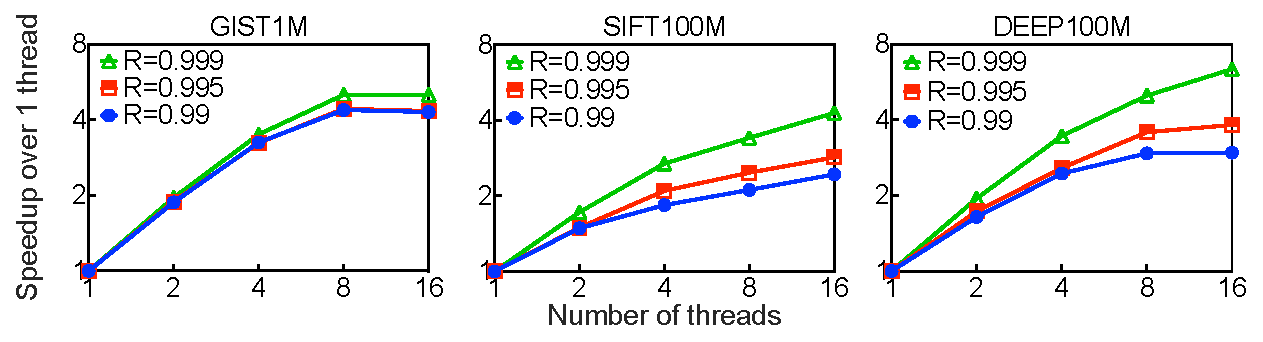
\includegraphics[width=0.48\textwidth]{figures/eva_speedup_Skylake}
    \caption[Speedups of \Hammer]{Speedups of \Hammer over the sequential baseline on Skylake.}
    \label{fig:eval-speedup-skylake}
\end{figure}

Figure~\ref{fig:eval-speedup-skylake} shows that \Hammer on Skylake achieves average $4.4\times$ and $5.2\times$ speedups over the sequential baseline with 8- and 16-thread at recall 0.999, respectively. 

\section{Comparison with a GPU Implementation.} 

\begin{table}[ht!]
\small
%\footnotesize
    \caption{Latency comparison of \Hammer and Faiss-GPU on five datasets. 
            \textmd{{\tt Lt.} means \emph{Latency}.
                    {\tt OOM} means \emph{out of memory}. 
                    Faiss-GPU's index format is IVFFLat.
                    \Hammer uses 32 threads.}}
    \label{tab:gpu_latency}
    \begin{tabular}{|c|cc|c|c|}
            \hline
            \multirow{2}{*}{Datasets} & \multicolumn{2}{c|}{Faiss-GPU w/ IVFFlat}                             & \multicolumn{2}{c|}{\Hammer-32T on KNL}                                    \\ \cline{2-5} 
            & \multicolumn{1}{c|}{R@100}  & \multicolumn{1}{c|}{Lt. (ms.)} & \multicolumn{1}{c|}{R@100} & \multicolumn{1}{c|}{Lt. (ms.)} \\ 
            \hline \hline
            SIFT1M                    & \multicolumn{1}{c|}{0.52}          & 0.87                               & \textbf{0.91}                              & \textbf{0.61}                               \\
            GIST1M                    & \multicolumn{1}{c|}{0.36}          & 7.25                               & \textbf{0.90}                              & \textbf{1.21}                               \\
            DEEP10M                   & \multicolumn{1}{c|}{0.62}          & 5.79                               & \textbf{0.90}                              & \textbf{0.96}                               \\
            SIFT100M                  & \multicolumn{1}{c|}{OOM} & \multicolumn{1}{c|}{OOM}              & \textbf{0.90}                              & \textbf{2.00}                               \\
            DEEP100M                  & \multicolumn{1}{c|}{OOM} & \multicolumn{1}{c|}{OOM}              & \textbf{0.90}                              & \textbf{1.91}                               \\ \hline
        \end{tabular}
\end{table}
%\section{Compare with a GPU Implementation.} 
We also compare \Hammer with a GPU-based large-scale ANNS algorithm~\cite{johnson2017billion} in the Faiss library~\cite{faiss-code}. The GPU experiments are conducted on an NVIDIA Tesla P100 with CUDA 10.2. Faiss is set to have one query in every batch because we focus on reducing the online query latency to meet stringent latency requirements.
Table~\ref{tab:gpu_latency} shows the latency comparison results on five datasets. \Hammer uses 32 threads on KNL.
For the SIFT100M and DEEP100M, Faiss-GPU complains of out-of-memory errors. 
For other datasets, \Hammer outperforms Faiss-GPU with $1.4\times$ to $6.0\times$ speedup and much better recall, which indicates that \Hammer can effectively achieve faster latency on CPUs than GPU-based algorithms.
%, which are often much cheaper than GPUs. 
% Please add the following required packages to your document preamble:
% \usepackage{multirow}
%\minjia{If space is a issue, let's put the comparison with GPU to the appendix.}



{
\section{Effects on memory bandwidth.}

\begin{figure}[h]
\centering
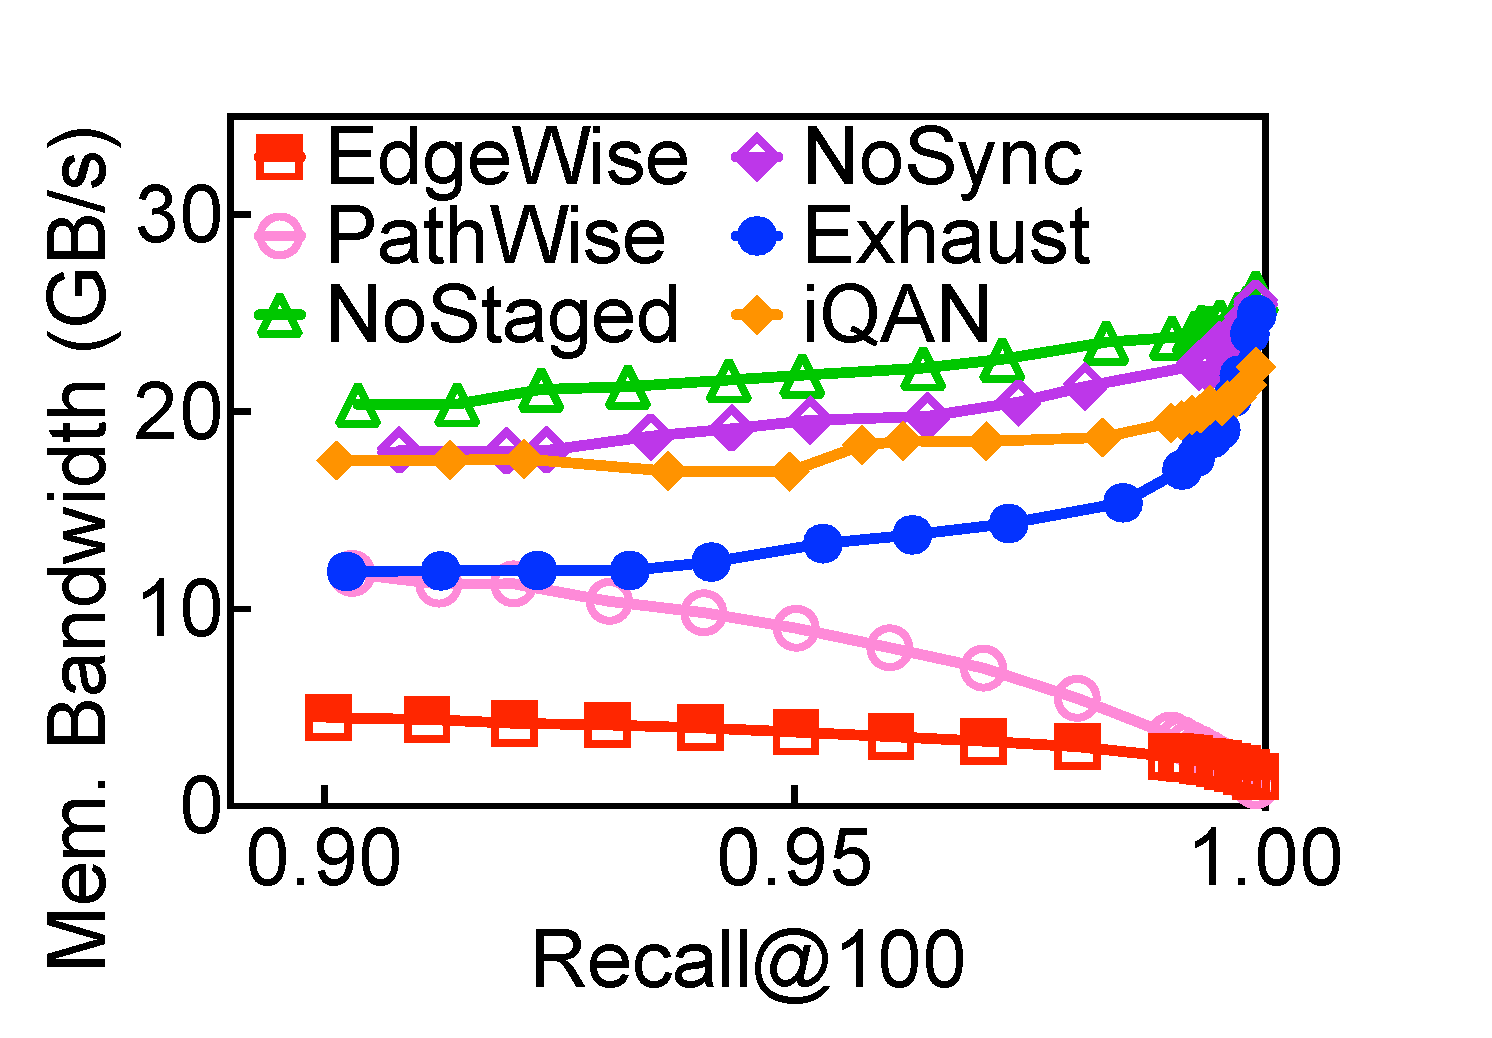
\includegraphics[width=0.35\textwidth]{figures/eva_mem_bandwidth_KNL}
\caption{Memory bandwidth on KNL using 32 threads.}
\label{fig:eva_mem_bandwidth_KNL}
\end{figure}

Figure~\ref{fig:eva_mem_bandwidth_KNL} shows that {\Hammer} achieves a much higher memory bandwidth utilization than \emph{EdgeWise}. For example, the memory bandwidth increases from 1.6~GB/s to 21.1~GB/s at recall 0.999. This bandwidth improvement comes from \Hammer's design to expose more parallelism during neighbor expansion while carefully eliminating synchronization overhead and redundant computations. 
To see how each optimization affects the memory bandwidth utilization, we also include the results of intermediate configurations. \emph{PathWise} overall achieves better memory bandwidth utilization than \emph{EdgeWise}. This is because it exposes more parallelism during the neighbor expansion process. However, as the recall target increases, the memory bandwidth of \emph{Pathwise} declines gradually towards \emph{EdgeWise}. This is because \emph{PathWise} does not apply redundancy-aware synchronization and still merges local candidates to the global priority queue in every iteration. As a result, the synchronization overhead becomes a dominant factor and limits the memory bandwidth utilization when the search is under the high recall region.
\emph{NoStaged}, \emph{NoSync}, \emph{Exhaust}, and \emph{iQAN} all improve the memory bandwidth utilization considerably because they all reduce frequent synchronizations.
\emph{NoStaged} and \emph{NoSync} have slightly higher memory bandwidth utilization than \Hammer because \emph{NoStaged} and \emph{NoSync} either use the maximum expansion width during the entire search process or perform no synchronization across worker threads, which leads to more (redundant) data loads during neighbor expansion. Therefore, \Hammer results in shorter query latency than \emph{NoStaged} and \emph{NoSync} even though it requires slightly less memory bandwidth utilization.  

% Compared to \emph{EdgeWise}, \Hammer improves the memory bandwidth utilization by $7.4\times$ on average for all recall cases because of its path-wise parallelism and redundancy-aware synchronization.
% Meanwhile, both \emph{NoStaged} and \emph{NoSync} have slightly higher memory bandwidth utilization than \Hammer. This is because \emph{NoStaged} and \emph{NoSync} either use the maximum expansion width during the entire search process or perform no synchronization across worker threads, which leads to more (redundant) data loads for neighbor expansion. Thus, \Hammer results in shorter query latency than  \emph{NoStaged} and \emph{NoSync} even though it requires slightly less memory bandwidth utilization.
% Moreover, \emph{Exhaust} have slightly higher memory bandwidth utilization than \Hammer for higher recall targets, and \emph{Pathwise}'s performance declines gradually towards \emph{EdgeWise}'s, which both show the significant impact synchronization has on memory bandwidth utilization, and by extension, on the latency.
}



%% Backup
%%%%%%%%%%%%%%%%%%%%%%%%%%%%%%%%%%%%